%\documentclass[handout]{beamer}
\documentclass[t,french]{beamer}
\usepackage{babel}
\usepackage[latin1]{inputenc}
\usepackage{graphicx} %for jpg files
\usepackage{beamerthemesplit} % new 
\usetheme[compress]{Berlin}
\usecolortheme{beaver}
\usepackage{tikz}%tikz figures
\usetikzlibrary{shapes}
\usepackage{pgffor}% http://ctan.org/pkg/pgffor
\usepackage{multirow}
\usepackage{ifthen}
\usepackage{subfigure} %spacing for table of contents
%\usepackage{multimedia} %videos inside frame
\usepackage{boolexpr}
\usepackage{movie15}
%\usepackage{bbold}
\usepackage{amsmath}
\usepackage{amsfonts}
\usepackage{amssymb}

\graphicspath{{images/}}

\def\R{ \ensuremath{\mathcal{R}} }
\def\C{ \ensuremath{\mathcal{C}} }
\def\SV{ \ensuremath{\mathcal{SV}} }

\setbeamercolor{alerted text}{fg=orange}
\setbeamercolor{background canvas}{bg=white}
\setbeamercolor{block body alerted}{bg=normal text.bg!90!black}
\setbeamercolor{block body}{bg=normal text.bg!90!black}
\setbeamercolor{block body example}{bg=normal text.bg!90!black}
\setbeamercolor{block title}{bg=blue}
\setbeamercolor{fine separation line}{}
\setbeamercolor{frametitle}{fg=black,bg=gray!30}
\setbeamercolor{item projected}{fg=black}
\setbeamercolor{normal text}{bg=black,fg=black}
\setbeamercolor{palette sidebar primary}{use=normal text,fg=normal text.fg}
\setbeamercolor{palette sidebar quaternary}{use=structure,fg=structure.fg}
\setbeamercolor{palette sidebar secondary}{use=structure,fg=structure.fg}
\setbeamercolor{palette sidebar tertiary}{use=normal text,fg=normal text.fg}
\setbeamercolor{section in sidebar}{fg=black}
\setbeamercolor{section in sidebar shaded}{fg= grey}
\setbeamercolor{separation line}{}
\setbeamercolor{sidebar}{bg=red}
\setbeamercolor{sidebar}{parent=palette primary}
\setbeamercolor{structure}{bg=black, fg=red}
\setbeamercolor{subsection in sidebar}{fg=black}
\setbeamercolor{subsection in sidebar shaded}{fg=grey}
\setbeamercolor{title}{fg=black!100,bg=gray!30}
\setbeamercolor{titlelike}{fg=brown}

%several template parameters
\setbeamertemplate{frametitle}[default][center]
\setbeamertemplate{blocks}[rounded][shadow=true]
%\beamertemplateshadingbackground{white!20}{black!20}
\setbeamertemplate{background canvas}[vertical shading][bottom=white,top=white!25]
\setbeamertemplate{sidebar canvas left}[horizontal shading][left=white!40!black,right=black]
\setbeamercolor{footline in sidebar}{fg=black}%[page number]
%\setbeamertemplate{footline}[frame number]
%suppress navigational bar
\beamertemplatenavigationsymbolsempty
%experimental stuff
\setbeamertemplate{title page}[default][rounded=true,shadow=true]


% Images
\pgfdeclareimage[width=10cm]{ROSEquation}{./images/ros_equation_2}
\pgfdeclareimage[width=10cm]{gazebo}{./images/gazebo_horz_cmyk_pos.jpg}
\pgfdeclareimage[width=10cm]{opencv}{./images/opencv_logo.png}
\pgfdeclareimage[width=10cm]{pcl}{./images/pointcloudlibrary_horz_large_pos.jpg}
\pgfdeclareimage[width=10cm]{moveit}{./images/moveit-logo.png}

% Tikz libraries
\usetikzlibrary{shadows}
\usetikzlibrary{automata}
\usetikzlibrary{arrows}

% For arrows
\definecolor{darkblue}{rgb}{0.2,0.2,0.6}
\definecolor{darkred}{rgb}{0.6,0.1,0.1}
\definecolor{darkgreen}{rgb}{0.2,0.6,0.2}

\def\arrowt{
  (0.1,0.5) -- (0.0,1) -- (6.0,1.0) [rounded corners=0.5] --
  (6.0,1.5) [rounded corners=1] -- (7.0,0.5) [rounded corners=0.5] --
  (6.0,-0.5) [sharp corners] -- (6.0,0.0) -- (0.0,0.0)
  [rounded corners=1] -- (0.1,0.5) -- cycle
}

\def\arrowd{
  (10.75:1.1) -- (6.5:1) arc (6.25:120:1) [rounded corners=0.5] --
  (120:0.9) [rounded corners=1] -- (130:1.1) [rounded corners=0.5] --
  (120:1.3) [sharp corners] -- (120:1.2) arc (120:5.25:1.2)
  [rounded corners=1] -- (10.75:1.1) -- (6.5:1) -- cycle
}

\def\arrow{
  (10.75:1.1) -- (6.5:1) arc (6.25:90:1) [rounded corners=0.5] --
  (90:0.9) [rounded corners=1] -- (100:1.1) [rounded corners=0.5] --
  (90:1.3) [sharp corners] -- (90:1.2) arc (90:5.25:1.2)
  [rounded corners=1] -- (10.75:1.1) -- (6.5:1) -- cycle
}

\def\arrowtd{
  (-10.75:1.1) -- (-6.5:1) arc (-6.25:-170:1) [rounded corners=0.5] --
  (-170:0.9) [rounded corners=1] -- (-180:1.1) [rounded corners=0.5] --
  (-170:1.3) [sharp corners] -- (-170:1.2) arc (-170:-5.25:1.2)
  [rounded corners=1] -- (-10.75:1.1) -- (-6.5:1) -- cycle
}

\tikzset{
  ashadow/.style={opacity=.25, shadow xshift=0.07, shadow yshift=-0.07},
}


\def\arrows[#1]{         
  \begin{scope}[scale=#1]
    \draw[color=darkred, %
    drop shadow={ashadow, color=red!60!black}] \arrow;

    %\draw[color=darkgreen, bottom color=green!90!black, top color=green!60, %
    %drop shadow={ashadow, color=green!60!black}] [rotate=120] \arrow;

    %\draw[color=darkblue, right color=blue, left color=blue!60, %
    %drop shadow={ashadow, color=blue!60!black}] [rotate=240] \arrow;

    % to hide the green shadow

  \end{scope}
}

\include{commands}

\setlength{\unitlength}{\textwidth}  % measure in textwidths
\begin{document}

\title{Introduction ROS}

\author{Olivier Stasse \\ LAAS-CNRS, Toulouse, France}
%-- \insertframenumber/\inserttotalframenumber}

\date{15-19/09/2014} 

\AtBeginSection[]
{
  \begin{frame}
    \frametitle{Table des mati�res}
    \tableofcontents[currentsection,
      hideothersubsections]
  \end{frame}
}
%%%%%%%%%%%%%%%%%%%%%%%%%%%%%%%%%%%%%%%%%%%%%%%%%%%%%%%%%%%%%%%%%%%%%%%%%%%%%%%
{
  \usebackgroundtemplate{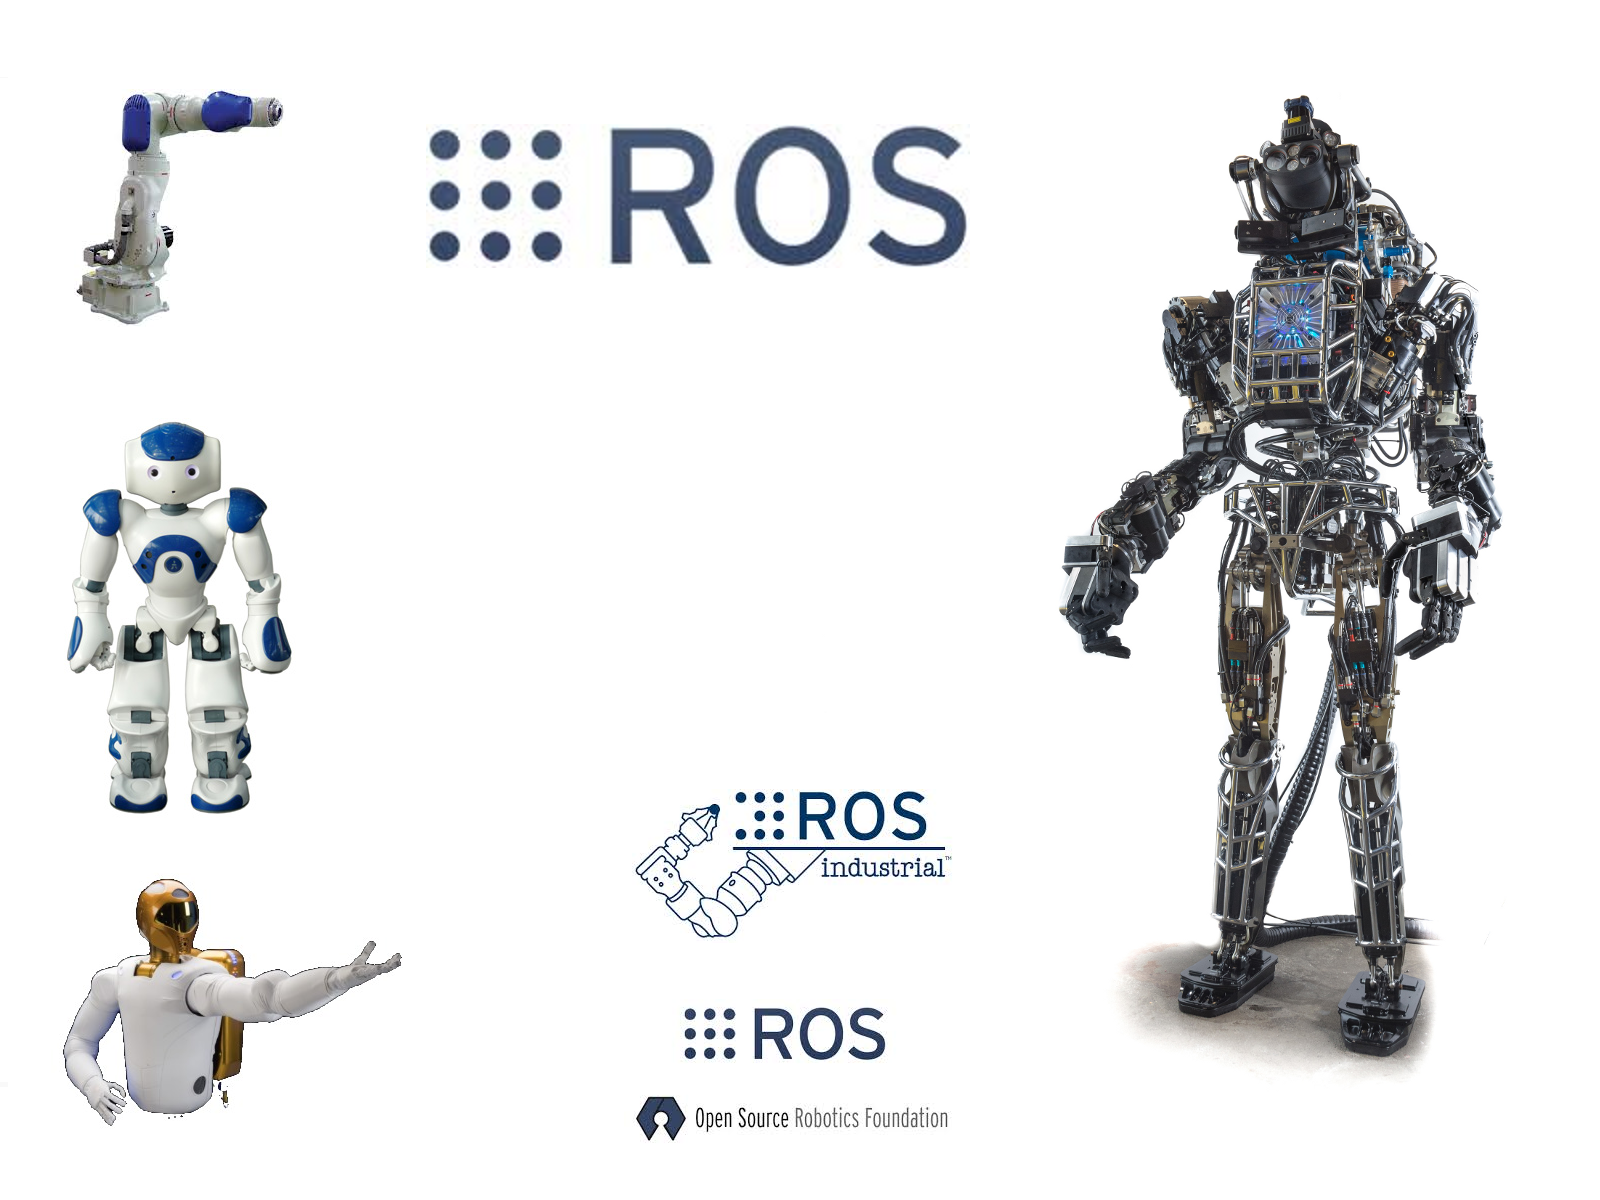
\includegraphics[width=1.0\paperwidth]{images/background-title-3.png}}
  \begin{frame}[plain]
    %\tikzstyle{stringbox}=[rectangle,color=black,fill=blue!10,text=black,draw,text opacity=0.4,align=flush center]
    \begin{tikzpicture}[remember picture, overlay]
       \node [yshift=1.8cm, xshift=-1cm, text width=6cm] (title) at (current page.center) 
            { Introduction � ROS \\
              Formation CNRS Entreprise};
       \node [xshift=-3.1cm,yshift=0.5cm,
              fill=white!10,fill opacity=0.7,right,text width=3cm]
             (author) at (current page.center) [scale=0.7]
            {
              Olivier STASSE, \\
              DR-2, CNRS, \\
              Gepetto, \\
              LAAS CNRS
            }; 
       \node [xshift=-3.1cm,yshift=-1.0cm,
              fill=white!10,fill opacity=0.7,
              right,text width=4cm]
        (author) 
        at (current page.center)
            {
              AIP, Toulouse\\
              Juin 2017
            }; 
    \end{tikzpicture}
  \end{frame}
}
\begin{frame}
  \frametitle{Table des mati�res}
  \tableofcontents[hideallsubsections]
\end{frame}


\section{Panorama}
%%%%%%%%%%%%%%%%%%%%%%%%%%%%%%%%%%%%%%%%%%%%%%%%%%%%%%%%%%%%%%%%%%%%%%%%%%%%%%%
\subsection{Motivations g�n�rales}
\begin{frame}
  \frametitle{Motivations - Application robotique \only<2>{- Outils}\only<3>{distribu�e}
  }
  
  \motivationpicture
  \motivationgraph
  \visible<1-2>{\logicalrelationship}
  \visible<2>{
    \implementationgraph
  }
  \visible<3>{
    \deploymentgraph
    \softwarerelationship
  }
\end{frame}
%
%%%%%%%%%%%%%%%%%%%%%%%%%%%%%%%%%%%%%%%%%%%%%%%%%%%%%%%%%%%%%%%%%%%%%%%%%%%%%%%%%
\begin{frame}
\frametitle{Motivations}
\begin{block}{Passage � l'�chelle}
La communaut� robotique doit \textit{collaborer} pour cr�er des syst�mes robotiques
de qualit� � l'exemple de l'informatique et la physique. \\
ROS est l'outil qui a permis ce passage. 
\end{block}

\begin{tikzpicture}[remember picture, overlay]
  \pgfputat{\pgfxy(0.0,-2.5)}{\pgfbox[left,base]{\pgfuseimage{ROSEquation}}};
  \node[xshift=3cm,yshift=-2.5cm]{Plomberie};
  \node[xshift=5cm,yshift=-2.5cm]{Outils};
  \node[xshift=7.15cm,yshift=-2.5cm]{Capacit�s};
  \node[xshift=9.21cm,yshift=-2.5cm]{Ecosyst�me};
\end{tikzpicture}
\end{frame}
%%%%%%%%%%%%%%%%%%%%%%%%%%%%%%%%%%%%%%%%%%%%%%%%%%%%%%%%%%%%%%%%%%%%%%%%%%%%%%%%%
\begin{frame}
  \frametitle{Motivations - Plomberie}
  \begin{block}{Middleware}
    \begin{itemize}     
      \item Publication/souscription � la transmission de messages anonymes (Message Passing)
      \item Enregistrer et rejouer des messages
      \item Requ�tes/r�ponses � des remote procedure calls
      \item Syst�me de param�tres distribu�s
    \end{itemize}
  \end{block}
\end{frame}
%%%%%%%%%%%%%%%%%%%%%%%%%%%%%%%%%%%%%%%%%%%%%%%%%%%%%%%%%%%%%%%%%%%%%%%%%%%%%%%%%
\begin{frame}
  \frametitle{Motivations - Outils}
  \begin{itemize}
    \item[rviz] Visualisateur graphique 3D.
    \item[rosbag] Enregistrement et visualisation des donn�es.
    \item[rxplot] Affichage en ligne.
    \item[rxgraph] Visualisation du syst�me.
    \item[rqt] Interface graphique de contr�le incr�mentale
    \item[catkin] Syst�me de compilation et de gestion de paquets.
  \end{itemize}
  \begin{tikzpicture}[remember picture,overlay]
    \visible<1-5>{\node at (2,-1.) {\pgfuseimage{rviz}};}
    \visible<2-5>{\node at (3.5,-1.) {\pgfuseimage{rosbag-slam}};}
    \visible<3-5>{\node at (5,-1.) {\pgfuseimage{rxplot}};}
    \visible<4-5>{\node at (6.5,-1.) {\pgfuseimage{rxgraph}};}
    \visible<5>{\node at (8,-1.) {\pgfuseimage{rqt}};}
  \end{tikzpicture}
\end{frame}
%%%%%%%%%%%%%%%%%%%%%%%%%%%%%%%%%%%%%%%%%%%%%%%%%%%%%%%%%%%%%%%%%%%%%%%%%%%%%%%%%
\begin{frame}
  \frametitle{Motivations - Ecosyst�me}
  \vskip 0.25cm
  \begin{itemize}
    \item D�finitions de messages standards pour les robots
    \item Librairie pour la g�om�trie des robots
    \item Language de description des robots
    \item Remote Procedure Calls pr�emptable
    \item Diagnostiques
    \item Estimation de pose
    \item Localisation
    \item Cartographie
    \item Navigation
  \end{itemize}
\end{frame}
%%%%%%%%%%%%%%%%%%%%%%%%%%%%%%%%%%%%%%%%%%%%%%%%%%%%%%%%%%%%%%%%%%%%%%%%%%%%%%%%%
\begin{frame}
  \frametitle{Motivations - Ecosyst�me}
  \begin{columns}[t]
    \begin{column}[T]{0.5\linewidth}
      \begin{itemize}
        \item Syst�mes d'exploitation
        \item Robots
        \item Packages
      \end{itemize}
    \end{column}
    \begin{column}[T]{0.5\linewidth}
      \visible<1>{\rosecosystem}
      \visible<2>{\robotsecosystem}
    \end{column}
  \end{columns}
\end{frame}
%%%%%%%%%%%%%%%%%%%%%%%%%%%%%%%%%%%%%%%%%%%%%%%%%%%%%%%%%%%%%%%%%%%%%%%%%%%%%%%%%
\subsection{ROS - Introduction}
%%%%%%%%%%%%%%%%%%%%%%%%%%%%%%%%%%%%%%%%%%%%%%%%%%%%%%%%%%%%%%%%%%%%%%%%%%%%%%%%%
\begin{frame}
\frametitle{ROS: Bref historique}
 \vskip -0.25cm
 {\footnotesize
 \begin{tabular}{|p{3cm}|p{7.5cm}|} \hline 
   2008 & D�marrage de ROS par Willow Garage \\ 
   2010 - Janvier & ROS 1.0 \\
   2010 - Mars & Box Turtle \\
   2010 - Aout & C Turtle \\
   2011 - Mars &  Diamondback \\
   2011 - Aout & Electric Emys \\
   2012 - Avril & Fuerte \\
   2012 - D�cembre & Groovy Galapagos\\
   2013 - F�vrier & Open Source Robotics Fundation poursuit la gestion de ROS \\
   2013 - Aout & Willow Garage est absorb� par Suitable Technologies \\
   2013 - Aout & Le support de PR-2 est repris par Clearpath Robotics\\
   2013 - Septembre& Hydro Medusa (pr�vu) \\ 
   2014 - Juillet & Indigo Igloo (EOL - Avril 2019)\\ 
   2015 - May & Jade Turtle (EOL - Mai 2017) \\
   2016 - May & Kinetic Kame (EOL - Mai 2021) \\ 
   2017 - May & Lunar Loggerhead \\ \hline
 \end{tabular}
 }
\end{frame}
%%%%%%%%%%%%%%%%%%%%%%%%%%%%%%%%%%%%%%%%%%%%%%%%%%%%%%%%%%%%%%%%%%%%%%%%%%%%%%%%%
\begin{frame}
\frametitle{ROS: Normalisation des releases}
 \vskip -0.25cm
 \begin{itemize}
   \item Kinetic Kame (Mai 2016 - Mai 2021)
     \begin{itemize}
       \item Ubuntu Wily (15.10)
       \item Ubuntu Xenial (16.04 LTS)
       \item C++11, Boost 1.55, Lisp SBCL 1.2.4, Python 2.7, CMake 3.0.2
       \item Ogre3D 1.9.x, Gazebo 7, PCL 1.7.x, OpenCV 3.1.x, Qt 5.3.x, PyQt5
     \end{itemize}
   \item Indigo Igloo (May 2014)
     \begin{itemize}
       \item Ubuntu Saucy (13.10)
       \item Ubuntu Trusty (14.04 LTS)
       \item C++03, Boost 1.53, Lisp SBCL 1.0.x, Python 2.7, (Test
         additionels contre Python 3.3 recommend�s) CMake 2.8.11
     \end{itemize}
   \item Lien vers la ROS Enhancement Proposal (REPs) :\\
     \url{http://www.ros.org/reps/rep-0003.html}
 \end{itemize}
\end{frame}
%%%%%%%%%%%%%%%%%%%%%%%%%%%%%%%%%%%%%%%%%%%%%%%%%%%%%%%%%%%%%%%%%%%%%%%%%%%%%%%%%
\subsection{Exemple}
%%%%%%%%%%%%%%%%%%%%%%%%%%%%%%%%%%%%%%%%%%%%%%%%%%%%%%%%%%%%%%%%%%%%%%%%%%%%%%%%%
\begin{frame}
  \frametitle{Exemple: Asservissement visuel}
  \framerosvisualservo
\end{frame}

\begin{frame}
  \frametitle{Exemple: Asservissement visuel - Topics}
  \framerosvisualservotopics
\end{frame}

\begin{frame}
  \frametitle{Exemple: Asservissement visuel - Topics - Params}
  \framerosvisualservoparams
\end{frame}

\begin{frame}
  \frametitle{Exemple: Asservissement visuel - Software bus}
  \framerosvisualservosoftwarebus
\end{frame}

%%%%%%%%%%%%%%%%%%%%%%%%%%%%%%%%%%%%%%%%%%%%%%%%%%%%%%%%%%%%%%%%%%%%%%%%%%%%%%%%%
\subsection{Installation ROS Indigo}
%%%%%%%%%%%%%%%%%%%%%%%%%%%%%%%%%%%%%%%%%%%%%%%%%%%%%%%%%%%%%%%%%%%%%%%%%%%%%%%%%
\begin{frame}{Installation de ROS - Indigo - Ubuntu 14.04.4 LTS}
\begin{tikzpicture}[remember picture, overlay]        
  \matrix[anchor=west] at (0,-2.5)
  {
    \node[roslist] (instros1) 
      {1 - Sp�cifications des sources.list}; \\
    \node[roscode] (instros2) 
      {sudo sh -c 'echo "deb http ://packages.ros.org/ros/ubuntu
       precise main" $>$ /etc/apt/sources.list.d/ros-latest.list'}; \\
    \node[roslist] 
      {2 - Sp�cifications des clefs}; \\
    \node[roscode] 
      {wget http ://packages.ros.org/ros.key -O - $|$ sudo apt-key add -};\\
    \node[roslist] 
      {3 - Mise � jour des listes de paquets};\\
    \node[roscode] 
      {sudo apt-get update}; \\
    \node[roslist] 
      {4 - Installation des paquets};\\
    \node[roscode] 
      {sudo apt-get install ros-indigo-desktop-full};\\
  };
\end{tikzpicture}  
\end{frame}
%%%%%%%%%%%%%%%%%%%%%%%%%%%%%%%%%%%%%%%%%%%%%%%%%%%%%%%%%%%%%%%%%%%%%%%%%%%%%%%%%
\subsection{Configuration ROS Indigo}
%%%%%%%%%%%%%%%%%%%%%%%%%%%%%%%%%%%%%%%%%%%%%%%%%%%%%%%%%%%%%%%%%%%%%%%%%%%%%%%%%
\begin{frame}{Configuration - Indigo - Ubuntu 14.04.4 LTS}
\begin{tikzpicture}[remember picture, overlay]        
  \matrix[anchor=west] at (0,-2.5)
  {
    \node[roslist] 
      {1 - Sp�cifications de ROS\_ROOT et ROS PACKAGE PATH }; \\
    \node[roscode] 
      {env $|$ grep ROS}; \\
    \node[roslist] 
      {2 - Ligne � ajouter au fichier .bashrc}; \\
    \node[roscode] 
      {source /opt/ros/indigo/setup.bash};\\
    \node[roslist] 
      {3 - Cr�ation de l'espace catkin};\\
    \node[roscode] 
      {mkdir -p \textasciitilde/catkin\_ws/src \\
       cd \textasciitilde/catkin\_ws/src \\
       catkin\_init\_workspace}; \\
    \node {\tiny Tutorial Installing and Confixguring Your ROS Environment :}; \\
    \node {\tiny \url{http://wiki.ros.org/ROS/Tutorials/InstallingandConfiguringROSEnvironment}}; \\
  };
\end{tikzpicture}  
\end{frame}
%%%%%%%%%%%%%%%%%%%%%%%%%%%%%%%%%%%%%%%%%%%%%%%%%%%%%%%%%%%%%%%%%%%%%%%%%%%%%%%%%
\begin{frame}{Configuration - Indigo - Ubuntu 14.04.4 LTS}
\begin{tikzpicture}[remember picture, overlay]        
  \matrix[anchor=west] at (0,-1.0)
  {
    \node[roslist] 
      {4 - Ligne � ajouter au fichier .bashrc}; \\
    \node[roscode] 
      {source \$HOME/catkin\_ws/devel/setup.bash}; \\
    \node {\tiny Tutorial Installing and Configuring Your ROS Environment :}; \\
    \node {\tiny \url{http://wiki.ros.org/ROS/Tutorials/InstallingandConfiguringROSEnvironment}}; \\
  };
\end{tikzpicture}  
\end{frame}
%%%%%%%%%%%%%%%%%%%%%%%%%%%%%%%%%%%%%%%%%%%%%%%%%%%%%%%%%%%%%%%%%%%%%%%%%%%%%%%%%
\begin{frame}{Configuration - Indigo - Ubuntu 14.04.4 LTS}
\begin{tikzpicture}[remember picture, overlay]        
  \matrix[anchor=west] at (0,-2.5)
  {
    \node[roslist] 
      { Votre distribution ROS est indiqu�e par ROS\_DISTRO }; \\
    \node[roscode] 
      {ROS\_DISTRO=indigo }; \\
    \node[roslist]
      { L'annuaire de votre application est sp�cifi� par ROS\_MASTER\_URI};\\
    \node[roscode] 
      {ROS\_MASTER\_URI=http://localhost:11311 \\
       ROS\_MASTER\_URI=http://hostname:port\_number \\}; \\
    \node[roslist]
      {\textbf{hostname} dans ROS\_MASTER\_URI indique l'ordinateur o� \textbf{roscore} est lanc�.
        \textbf{port\_number} indique le port o� \textbf{roscore} attend les connections. 
      };\\
  };
\end{tikzpicture}  
\end{frame}

%%%%%%%%%%%%%%%%%%%%%%%%%%%%%%%%%%%%%%%%%%%%%%%%%%%%%%%%%%%%%%%%%%%%%%%%%%%%%%%%%
\subsection{Navigation dans ROS Indigo}
%%%%%%%%%%%%%%%%%%%%%%%%%%%%%%%%%%%%%%%%%%%%%%%%%%%%%%%%%%%%%%%%%%%%%%%%%%%%%%%%%
\begin{frame}{ROS Filesystem - Navigation - Indigo}
\begin{tikzpicture}[remember picture, overlay]        
  \matrix[anchor=west] at (0,-3.0)
  {
    \node[roslist] 
      {1 - rospack : Donne les informations sur les paquets (exemple roscpp)}; \\
    \node[roscode] 
      {rospack find roscpp}; \\
    \node[roslist] 
      {2 - roscd : Bascule le r�pertoire directement sur le paquet}; \\
    \node[roscode] 
      {roscd roscpp \\
       roscd roscpp/cmake \\
       roscd log};\\
    \node[roslist] 
      {3 - rosls : Affiche le contenu du r�pertoire d'un paquet};\\
    \node[roscode] 
      {rosls roscpp\_tutorials}; \\
    \node {\tiny Tutorial Navigation dans le syst�me de fichiers }; \\
    \node {\tiny \url{http://wiki.ros.org/ROS/Tutorials/NavigatingTheFilesystem}}; \\
  };
\end{tikzpicture}  
\end{frame}
%%%%%%%%%%%%%%%%%%%%%%%%%%%%%%%%%%%%%%%%%%%%%%%%%%%%%%%%%%%%%%%%%%%%%%%%%%%%%%%%%
\subsection{Cr�ation d'un paquet pour ROS Indigo}    
%%%%%%%%%%%%%%%%%%%%%%%%%%%%%%%%%%%%%%%%%%%%%%%%%%%%%%%%%%%%%%%%%%%%%%%%%%%%%%%%%
\begin{frame}{Cr�ation d'un paquet ROS - D�finition - Indigo}
  \begin{itemize}
    \item Le paquet doit contenir un fichier \textcolor{blue}{package.xml} qui suit le
      format catkin. Le fichier \textcolor{blue}{package.xml} contient des meta
      informations sur le paquet.
    \item Il n'y a qu'un seul paquet par r�pertoire. \\
      Les paquets imbriqu�s, et les paquets dans un m�me
      r�pertoire sont interdits.
  \end{itemize}
  Le paquet le plus simple est:
  \begin{tikzpicture}   
    \node[roscode]
      {mon\_paquet/\\
       CMakeLists.txt\\
       package.xml};
  \end{tikzpicture}
\end{frame}
%%%%%%%%%%%%%%%%%%%%%%%%%%%%%%%%%%%%%%%%%%%%%%%%%%%%%%%%%%%%%%%%%%%%%%%%%%%%%%%%%
\section{Organisation des programmes sous ROS}
%%%%%%%%%%%%%%%%%%%%%%%%%%%%%%%%%%%%%%%%%%%%%%%%%%%%%%%%%%%%%%%%%%%%%%%%%%%%%%%%%
\subsection{Cr�ation de paquets}
%%%%%%%%%%%%%%%%%%%%%%%%%%%%%%%%%%%%%%%%%%%%%%%%%%%%%%%%%%%%%%%%%%%%%%%%%%%%%%%%%
\begin{frame}{Paquets dans un workspace catkin - (1/9) - Indigo}
\tikzstyle{every node}=[anchor=west
%,font=\fontsize{6}{6}\selectfont
]
\tikzstyle{selected}=[draw=blue!50,fill=blue!20
%,font=\fontsize{6}{6}\selectfont
]
\tikzstyle{root}=[draw=blue,fill=blue!50
%,font=\fontsize{6}{6}\selectfont
]
{\scriptsize
\begin{tikzpicture}[%
  grow via three points={one child at (0.75,-0.5) and
  two children at (0.75,-0.5) and (0.75,-1.0)},
  edge from parent path={(\tikzparentnode.south) |- (\tikzchildnode.west)}]
  \node [root] {work\_space\_folder}
    child {  node [selected] {src}
      child { node {CMakeLists.txt}}
      child { node [selected] {package\_1}
        child { node {CMakeLists.txt}}
        child { node {package.xml}}
      }
     child [missing] {}				
     child [missing] {}
     child { node [selected] {...}}
     child { node [selected] {package\_n}
        child { node {CMakeLists.txt}}
        child { node {package.xml}}
      }
    };
\end{tikzpicture}
}
\end{frame}
%%%%%%%%%%%%%%%%%%%%%%%%%%%%%%%%%%%%%%%%%%%%%%%%%%%%%%%%%%%%%%%%%%%%%%%%%%%%%%%%%
\begin{frame}{Paquets dans un workspace catkin - (2/9) - Indigo}
\begin{tikzpicture}[remember picture, overlay]        
  \matrix[anchor=west] at (0,-2.5)
  {
    \node[roslist] 
      {1 - Aller dans le r�pertoire src du paquet}; \\
    \node[roscode] 
      {cd \textasciitilde/catkin\_ws/src}; \\
    \node[roslist]
    {Pour cr�er un nouveau package, et ses d�pendences:\\
      {\bf catkin\_create\_pkg}}; \\
    \node[roscode]
    {catkin\_create\_pkg beginner\_tutorials std\_msgs rospy roscpp\\
     catkin\_create\_pkg [package\_name] [depend1] [depend2] [depend3]};\\
  };
\end{tikzpicture}  
\end{frame}
%%%%%%%%%%%%%%%%%%%%%%%%%%%%%%%%%%%%%%%%%%%%%%%%%%%%%%%%%%%%%%%%%%%%%%%%%%%%%%%%%
\begin{frame}{Paquets dans un workspace catkin - (3/9) - Indigo}
\begin{tikzpicture}[remember picture, overlay]        
  %\draw[help lines] (0,-3) grid (5,0);         
  %\node at (0,0) {(0,0)};
  \matrix[anchor=west] at (0,-2.5)
  {
    \node[roslist] 
      {2 - D�pendences du premier ordre}; \\
    \node[roscode] 
      {rospack depends1 beginner\_tutorials}; \\
    \node {\footnotesize D�pendences standards: std\_msgs rospy roscpp };\\
    \node[roslist]
    {3 - Les d�pendences sont stock�es dans le fichier package.xml}; \\
    \node[roscode]
    {roscd beginner\_tutorials\\
     cat package.xml};\\
    \node[roslist]
    { \footnotesize
      $<$package$>$\\
      ...\\
      $<$buildtool\_depend$>$catkin$<$/buildtool\_depend$>$\\
      $<$build\_depend$>$roscpp$<$/build\_depend$>$\\
      ...\\
      $<$/package$>$
    };\\
  };
\end{tikzpicture}  
\end{frame}
%%%%%%%%%%%%%%%%%%%%%%%%%%%%%%%%%%%%%%%%%%%%%%%%%%%%%%%%%%%%%%%%%%%%%%%%%%%%%%%%%
\begin{frame}{Paquets dans un workspace catkin - (4/9) - Indigo}
\begin{tikzpicture}[remember picture, overlay]        
  %\draw[help lines] (0,-3) grid (5,0);         
  %\node at (0,0) {(0,0)};
  \matrix[anchor=west] at (0,-2.5)
  {
    \node[roslist] 
      {4 - D�pendences indirectes d'un paquet}; \\
    \node[roscode] 
      {rospack depends beginner\_tutorials}; \\
    \node[roslist]
    { \footnotesize$<$package$>$\\
      cpp\_common\\
      rostime\\
      roscpp\_traits\\
      roscpp\_serialization\\
      ...\\
      roslib\\
     rospy \\
      $<$/package$>$
    };\\
  };
\end{tikzpicture}  
\end{frame}
%%%%%%%%%%%%%%%%%%%%%%%%%%%%%%%%%%%%%%%%%%%%%%%%%%%%%%%%%%%%%%%%%%%%%%%%%%%%%%%%%
\begin{frame}{Personnalisation du paquet - (5/9) - Indigo}
\begin{tikzpicture}[remember picture, overlay]        
  %\draw[help lines] (0,-3) grid (5,0);         
  %\node at (0,0) {(0,0)};
  \matrix[anchor=west] at (0,-2.5)
  {
    \node[roslist] 
      {5 - Description du paquet}; \\
    \node[roscode] 
      {$<$description$>$The beginner\_tutorials package$<$/description$>$}; \\
    \node[roscode]
    { \footnotesize$<$package$>$\\
      $<$!- One maintainer tag required, multiple allowed, one person per tag -$>$ \\
      $<$!- Exemple : -$>$ \\
      $<$!- $<$maintainer email="jane.doe@example.com"$>$Jane Doe$<$/maintainer$>$ -$>$ \\
      $<$maintainer email="user@todo.todo"$>$user$<$/maintainer$>$\\
    };\\
  };
\end{tikzpicture}  
\end{frame}
%%%%%%%%%%%%%%%%%%%%%%%%%%%%%%%%%%%%%%%%%%%%%%%%%%%%%%%%%%%%%%%%%%%%%%%%%%%%%%%%%
\begin{frame}{Personnalisation du paquet - (6/9) - Indigo}
\begin{tikzpicture}[remember picture, overlay]        
  %\draw[help lines] (0,-3) grid (5,0);         
  %\node at (0,0) {(0,0)};
  \matrix[anchor=west] at (0,-2.5)
  {
    \node[roslist]{7 - License du paquet}; \\
    \node[roscode] 
      {
        $<$!- One license tag required, multiple allowed, one license per tag -$>$ \\
        $<$!- Commonly used license strings : -$>$\\
        $<$!- BSD, MIT, Boost Software License, GPLv2, GPLv3, LGPLv2.1,LGPLv3 -$>$\\
        $<$license$>$TODO$<$/license$>$ }; \\
    \node[roslist]{La license souvent utilis�e sous ROS est la BSD};\\
    \node[roscode]{ $<$license$>$BSD$<$/license$>$ };\\
  };
\end{tikzpicture}  
\end{frame}
%%%%%%%%%%%%%%%%%%%%%%%%%%%%%%%%%%%%%%%%%%%%%%%%%%%%%%%%%%%%%%%%%%%%%%%%%%%%%%%%%
\begin{frame}{Personnalisation du paquet - (7/9) - Indigo}
\begin{tikzpicture}[remember picture, overlay]        
  %\draw[help lines] (0,-3) grid (5,0);         
  %\node at (0,0) {(0,0)};
  \matrix[anchor=west] at (0,-2.5)
  {
    \node[roslist]{8 - Sp�cification des d�pendences}; \\
    \node[roscode] 
      {\tiny $<$!- The * depend tags are used to specify dependencies -$>$ \\
       $<$!- Dependencies can be catkin packages or system dependencies -$>$ \\
       $<$!- Exemples : -$>$ \\
       $<$!- Use build\_depend for packages you need at compile time : -$>$ \\
       $<$!- $<$build\_depend$>$genmsg$<$/build\_depend$>$ -$>$\\
       $<$!- Use buildtool\_depend for build tool packages : -$>$\\
       $<$!- $<$buildtool\_depend$>$catkin$<$/buildtool\_depend$>$ -$>$\\
       $<$!- Use run\_depend for packages you need at runtime : -$>$\\
       $<$!- $<$run\_depend$>$python-yaml$<$/run\_depend$>$ -$>$\\
       $<$!- Use test depend for packages you need only for testing : -$>$\\
       $<$!- $<$test depend$>$gtest$<$/test depend$>$ -$>$\\
       $<$buildtool\_depend$>$catkin$<$/buildtool\_depend$>$\\
       $<$build\_depend$>$roscpp$<$/build\_depend$>$\\
       $<$build\_depend$>$rospy$<$/build\_depend$>$\\
       $<$build\_depend$>$std\_msgs$<$/build\_depend$>$ }; \\
  };
\end{tikzpicture}  
\end{frame}
%%%%%%%%%%%%%%%%%%%%%%%%%%%%%%%%%%%%%%%%%%%%%%%%%%%%%%%%%%%%%%%%%%%%%%%%%%%%%%%%%
\begin{frame}{Personnalisation du paquet - (8/9) - Indigo}
\begin{tikzpicture}[remember picture, overlay]        
  %\draw[help lines] (0,-3) grid (5,0);         
  %\node at (0,0) {(0,0)};
  \matrix[anchor=west] at (0,-2.5)
  {
    \node[roslist]{9 - Ajout de la d�pendence � l'ex�cution:}; \\
    \node[roscode] 
      { 
        $<$buildtool\_depend$>$catkin$<$/buildtool\_depend$>$\\
        $<$build\_depend$>$roscpp$<$/build\_depend$>$\\
        $<$build\_depend$>$rospy$<$/build\_depend$>$\\
        $<$build\_depend$>$std\_msgs$<$/build\_depend$>$\\
        $<$run\_depend$>$roscpp$<$/run\_depend$>$\\
        $<$run\_depend$>$rospy$<$/run\_depend$>$\\
        $<$run\_depend$>$std\_msgs$<$/run\_depend$>$
      }; \\
  };
\end{tikzpicture}  
\end{frame}
%%%%%%%%%%%%%%%%%%%%%%%%%%%%%%%%%%%%%%%%%%%%%%%%%%%%%%%%%%%%%%%%%%%%%%%%%%%%%%%%%
\begin{frame}{Personnalisation du paquet - (9/9) - Indigo}
\begin{tikzpicture}[remember picture, overlay]        
  %\draw[help lines] (0,-3) grid (5,0);         
  %\node at (0,0) {(0,0)};
  \matrix[anchor=west] at (0,-2.5)
  {
    \node[roslist]{10 - Fichier \textcolor{blue}{package.xml} final}; \\
    \node[roscode] 
      { \tiny 
        $<$?xml version="1.0" ?$>$ \\
        $<$package$>$ \\
        $<$name$>$beginner\_tutorials$<$/name$>$\\
        $<$version$>$0.1.0$<$/version$>$ \\
        $<$description$>$The beginner tutorials package$<$/description$>$ \\
        $<$maintainer email="you@yourdomain.tld"$>$Your Name$<$/maintainer$>$\\
        $<$license$>$BSD$<$/license$>$ \\
        $<$url type="website"$>$http ://wiki.ros.org/beginner tutorials$<$/url$>$ \\
        $<$author email="you@yourdomain.tld"$>$Jane Doe$<$/author$>$ \\
        $<$buildtool\_depend$>$catkin$<$/buildtool\_depend$>$ \\
        $<$build\_depend$>$roscpp$<$/build\_depend$>$ \\
        $<$build\_depend$>$rospy$<$/build\_depend$>$ \\
        $<$build\_depend$>$std\_msgs$<$/build\_depend$>$ \\
        $<$run\_depend$>$roscpp$<$/run\_depend$>$ \\
        $<$run\_depend$>$rospy$<$/run\_depend$>$ \\
        $<$run\_depend$>$std\_msgs$<$/run\_depend$>$ \\
        $<$/package$>$
      }; \\
  };
\end{tikzpicture}  
\end{frame}
%%%%%%%%%%%%%%%%%%%%%%%%%%%%%%%%%%%%%%%%%%%%%%%%%%%%%%%%%%%%%%%%%%%%%%%%%%%%%%%%%
\begin{frame}{Compilation des paquets Indigo}
  \begin{tikzpicture}[remember picture, overlay]
    \matrix[anchor=west] at (0,-2.5)
    {
      \node[roslist]{
        La compilation de tous les paquets s'effectue avec une seule commande.\\
        Cette commande doit s'effectuer dans le r�pertoire du workspace.\\
        Le r�pertoire {\bf build} du workspace stocke les objets compil�s interm�diaires.\\
        Le r�pertoire {\bf devel} du workspace stocke les ex�cutables et les
        librairies compil�es.\\
      };\\
      \node[roscode]{
        catkin\_make \\
        catkin\_make install\\
      };\\
    };
  \end{tikzpicture}
\end{frame}
%%%%%%%%%%%%%%%%%%%%%%%%%%%%%%%%%%%%%%%%%%%%%%%%%%%%%%%%%%%%%%%%%%%%%%%%%%%%%%%%%
\subsection{D�finitions}
%%%%%%%%%%%%%%%%%%%%%%%%%%%%%%%%%%%%%%%%%%%%%%%%%%%%%%%%%%%%%%%%%%%%%%%%%%%%%%%%%
\begin{frame}{Graphe d'applications avec ROS}
  \begin{itemize}
    \item[Nodes]: Un node est un ex�cutable qui utilise ROS pour communiquer 
      avec d'autres noeuds.     
    \item[Messages]: Types de donn�es ROS utilis�s pour souscrire ou publi� sur un topic.
    \item[Topics]: Les nodes peuvent \textit{publier} des messages sur un topic 
      aussi bien que \textit{souscrire} � un topic pour recevoir des messages.
    \item[Master]: Nom du service pour ROS (i.e. aide les noeuds � se trouver
      mutuellement).
    \item[{\footnotesize Param�tres}]: Informations tr�s peu dynamiques qui doivent �tre partag�s
      dans l'application.
    \item[rosout]: Equivalent de stdout/stderr.
    \item[roscore]: Master+rosout+parameter server (serveur de param�tres,
      introduit plus tard).
  \end{itemize}
\end{frame}
%%%%%%%%%%%%%%%%%%%%%%%%%%%%%%%%%%%%%%%%%%%%%%%%%%%%%%%%%%%%%%%%%%%%%%%%%%%%%%%%%
\begin{frame}{D�finitions - Node}
  \begin{itemize}
    \item Un fichier �xecutable dans un paquet ROS. 
    \item Les noeuds ROS utilisent une librairie client pour communiquer avec 
      les autres noeuds.
    \item Les noeuds peuvent \textbf{publier} ou \textbf{souscrire} � des 
      \textbf{topics}.
    \item Les noeuds peuvent fournir ou utiliser un \textbf{service}.
    \item Les librairies client sont :
      \begin{itemize}
        \item \textit{rospy} pour python.
        \item \textit{roscpp} pour C++.
      \end{itemize}
  \end{itemize}
\end{frame}

%%%%%%%%%%%%%%%%%%%%%%%%%%%%%%%%%%%%%%%%%%%%%%%%%%%%%%%%%%%%%%%%%%%%%%%%%%%%%%%%%
\section{Communications ROS}
%%%%%%%%%%%%%%%%%%%%%%%%%%%%%%%%%%%%%%%%%%%%%%%%%%%%%%%%%%%%%%%%%%%%%%%%%%%%%%%%%
\subsection{roscore}
%%%%%%%%%%%%%%%%%%%%%%%%%%%%%%%%%%%%%%%%%%%%%%%%%%%%%%%%%%%%%%%%%%%%%%%%%%%%%%%%%
\begin{frame}{Le syst�me des Name services}
  \begin{tikzpicture}[remember picture, overlay]
    \matrix[anchor=west] at (0,-2.5)
      {
        \node[roslist]
        {Pour pouvoir localiser et interagir entre les nodes il faut un \textbf{annuaire}.\\
        C'est le r�le de \textbf{roscore}.};\\
        \node[roslist]
        {Il doit �tre lanc� \textit{syst�matiquement} mais une seule fois.\\
         Si \textbf{roscore} ne se lance pas, il faut :
         \begin{itemize}
           \item V�rifier la connection r�seau.
           \item Si roscore ne s'initialise pas et �voque un probl�me de droits, 
            il faut v�rifier les droits sur le r�pertoire .ros
         \end{itemize}
        };\\
        \node[roslist]
        { \tiny
           Tutorial Understanding ROS Nodes : \url{http://wiki.ros.org/ROS/Tutorials/UnderstandingNodes}
        };\\
     };
  \end{tikzpicture}
\end{frame}
%%%%%%%%%%%%%%%%%%%%%%%%%%%%%%%%%%%%%%%%%%%%%%%%%%%%%%%%%%%%%%%%%%%%%%%%%%%%%%%%%
\begin{frame}{Le syst�me des Name services}
  \begin{tikzpicture}[remember picture, overlay]
    \matrix[anchor=west] at (0,-2.5)
      {
        \node[roslist]
        {Pour obtenir la liste des nodes actifs :};\\
        \node[roscode]
        {rosnode list};\\
        \node[roslist]
        {Pour obtenir des informations sur un node :};\\
        \node[roscode]
        {rosnode info /rosout};\\
         \node[roslist]
        {\tiny Tutorial Understanding ROS Nodes : \url{http://wiki.ros.org/ROS/Tutorials/UnderstandingNodes}};\\
      };
   \end{tikzpicture}
\end{frame}
%%%%%%%%%%%%%%%%%%%%%%%%%%%%%%%%%%%%%%%%%%%%%%%%%%%%%%%%%%%%%%%%%%%%%%%%%%%%%%%%%
\subsection{rosrun}
%%%%%%%%%%%%%%%%%%%%%%%%%%%%%%%%%%%%%%%%%%%%%%%%%%%%%%%%%%%%%%%%%%%%%%%%%%%%%%%%%
\begin{frame}{Utilisation de rosrun}
  \begin{tikzpicture}[remember picture, overlay]
    \matrix[anchor=west] at (0,-2.5)
      {
        \node[roslist]
        {Pour pouvoir lancer un fichier ex�cutable/node d'un paquet}; \\
        \node[roscode]
        {rosrun [package\_name][node\_name]}; \\
        \node[roslist]
        {Par exemple pour lancer turtlesim :}; \\
        \node[roscode]
        {rosrun turtlesim turtlesim\_node}; \\
        \node[roslist]
        {Pour renommer des arguments (utiliser rosnode list pour v�rifier) :};\\
        \node[roscode]
        {rosrun turtlesim turtlesim\_node --name:=my\_turtle};\\
        \node[roslist]
        {Pour tester si le node est actif};\\
        \node[roscode]
        {rosnode ping my\_turtle};\\
        \node[roslist]
        {\tiny Tutorial Understanding ROS Nodes : \url{http://wiki.ros.org/ROS/Tutorials/UnderstandingNodes}};\\
      };
   \end{tikzpicture}
\end{frame}
%%%%%%%%%%%%%%%%%%%%%%%%%%%%%%%%%%%%%%%%%%%%%%%%%%%%%%%%%%%%%%%%%%%%%%%%%%%%%%%%%
\begin{frame}{Comprendre les topics - Pr�paration}
  \begin{tikzpicture}[remember picture, overlay]
    \matrix[anchor=west] at (0,-2.5)
      {
        \node[roslist]
        {Pour d�marrer turtle\_sim et turtle\_teleop\_key};\\
        \node[roscode]
        {rosrun turtlesim turtlesim\_node\\
         rosrun turtlesim turtle\_teleop\_key};\\
        \node[roslist]
        {D�marrer le graphe de l'application :};\\
        \node[roscode]
        {rosrun rqt\_graph rqt\_graph};\\
        \node[roslist]
        {D�marrer le graphe de l'affichage des topics:};\\
        \node[roscode]
        {rosrun rqt\_plot rqt\_plot};\\
        \node[roslist]
        {\tiny Tutorial Understanding ROS Topics : \url{http://wiki.ros.org/ROS/Tutorials/UnderstandingTopics}};\\
      };
   \end{tikzpicture}
\end{frame}
%%%%%%%%%%%%%%%%%%%%%%%%%%%%%%%%%%%%%%%%%%%%%%%%%%%%%%%%%%%%%%%%%%%%%%%%%%%%%%%%%
\subsection{rostopic}
%%%%%%%%%%%%%%%%%%%%%%%%%%%%%%%%%%%%%%%%%%%%%%%%%%%%%%%%%%%%%%%%%%%%%%%%%%%%%%%%%
\begin{frame}{Comprendre les topics - \textbf{rostopic}}
  \begin{tikzpicture}[remember picture, overlay]
    \matrix[anchor=west] at (0,-2.5)
      {
        \node[roslist]
        {Les topics sont des donn�es \textbf{publi�es} par des noeuds,
        et auquelles les noeuds \textbf{souscrivent}.\\
        L'ex�cutable permettant d'avoir des informations sur les topics
        est \textbf{rostopic}.};\\
        \node[roscode]
        {rostopic bw display bandwith used by topic\\
         rostopic echo print messages to screen\\
         rostopic hz display publishing rate of topic\\
         rostopic list print information about active topics\\
         rostopic pub publish data to topic\\
         rostopic type print topic type
        };\\
        \node[roslist]
        {\tiny Tutorial Understanding ROS Topics : \url{http://wiki.ros.org/ROS/Tutorials/UnderstandingTopics}};\\
      };
   \end{tikzpicture}
\end{frame}
%%%%%%%%%%%%%%%%%%%%%%%%%%%%%%%%%%%%%%%%%%%%%%%%%%%%%%%%%%%%%%%%%%%%%%%%%%%%%%%%%
\subsection{roswtf}
%%%%%%%%%%%%%%%%%%%%%%%%%%%%%%%%%%%%%%%%%%%%%%%%%%%%%%%%%%%%%%%%%%%%%%%%%%%%%%%%%
\begin{frame}{V�rifier son installation ros - \textbf{roswtf}}
  Ce programme v�rifie l'installation de ROS et analyse les probl�mes.
  \begin{itemize}       
    \item Effectue le test suivant le r�pertoire.
    \item V�rifie la coh�rence de l'installation : variables d'environnements,
      paquets install�s.
    \item Analyse le graphe en cours d'ex�cution.
  \end{itemize}
  {\tiny Tutorial Getting started with roswtf : \url{http://wiki.ros.org/ROS/Tutorials/Getting\%20started\%20with\%20roswtf}};
\end{frame}
%%%%%%%%%%%%%%%%%%%%%%%%%%%%%%%%%%%%%%%%%%%%%%%%%%%%%%%%%%%%%%%%%%%%%%%%%%%%%%%%%
\subsection{rqt\_console}
%%%%%%%%%%%%%%%%%%%%%%%%%%%%%%%%%%%%%%%%%%%%%%%%%%%%%%%%%%%%%%%%%%%%%%%%%%%%%%%%%
\begin{frame}{rqt - \textbf{rqt\_console}}
  \begin{tikzpicture}[remember picture, overlay]
    \matrix[anchor=west] at (0,-2.5)
      {
        \node[roslist]
        {\textbf{rqt} est une interface d'affichage non 3D qui se peuple avec des plugins. 
          Elle permet de construire une interface de contr�le incr�mentalement.
          L'ex�cutable permettant d'afficher les messages des noeuds de fa�on centralis� 
          est \textbf{rqt\_console}.};\\
        \node[roscode]
        { rosrun rqt\_console rqt\_console \\
          rosrun rqt\_logger\_level rqt\_logger\_level
        };\\
        \node[roslist]
        {\tiny Tutorial Using rqt console et roslaunch \url{http://wiki.ros.org/ROS/Tutorials/UsingRqtconsoleRoslaunch}};\\
      };

  \end{tikzpicture}
\end{frame}
%%%%%%%%%%%%%%%%%%%%%%%%%%%%%%%%%%%%%%%%%%%%%%%%%%%%%%%%%%%%%%%%%%%%%%%%%%%%%%%%%
\subsection{roslaunch}
%%%%%%%%%%%%%%%%%%%%%%%%%%%%%%%%%%%%%%%%%%%%%%%%%%%%%%%%%%%%%%%%%%%%%%%%%%%%%%%%%
\begin{frame}{Lancer plusieurs noeuds - \textbf{roslaunch}}
  \begin{tikzpicture}[remember picture, overlay]
    \matrix[anchor=west] at (0,-2.5)
      {
        \node[roslist]
        {\textbf{roslaunch} lit un fichier xml qui contient tous les param�tres
          pour lancer une application distribu�e ROS.};\\
        \node[roscode]
        {roslaunch [package] [filename.launch]};\\
        \node[roslist]
        {Exemple :};\\
        \node[roscode]
        {roscd beginner\_tutorials\\
          roslaunch beginner\_tutorials turtlemimic.launch
        };\\
        \node[roslist]
        {\tiny Tutorial Using rqt console et roslaunch \url{http://wiki.ros.org/ROS/Tutorials/UsingRqtconsoleRoslaunch}};\\
      };
  \end{tikzpicture}
\end{frame}
%%%%%%%%%%%%%%%%%%%%%%%%%%%%%%%%%%%%%%%%%%%%%%%%%%%%%%%%%%%%%%%%%%%%%%%%%%%%%%%%%
\subsection{rosed}
%%%%%%%%%%%%%%%%%%%%%%%%%%%%%%%%%%%%%%%%%%%%%%%%%%%%%%%%%%%%%%%%%%%%%%%%%%%%%%%%%
\begin{frame}{Sp�cifier l'�diteur pour ROS - \textbf{rosed}}
  \begin{tikzpicture}[remember picture, overlay]
    \matrix[anchor=west] at (0,-2.5)
      {
        \node[roslist]
        {\textbf{roslaunch} permet d'�diter un fichier directement par le nom du paquet
          et non par le chemin entier. Il inclut la compl�tion par $<$Tab$>$.};\\
        \node[roscode]
        {rosed [package] [filename]};\\
        \node[roslist]
        {Exemple :};\\
        \node[roscode]
        {rosed roscpp Logger.msg};      \\
        \node[roslist]
        {L'�diteur utilis� est sp�cifi� par la variable d'environnement EDITOR};\\
        \node[roscode]
        {export EDITOR='emacs'};\\
        \node[roslist]
        {\tiny Tutorial Using rosed to edit files in ROS \url{http://wiki.ros.org/ROS/Tutorials/UsingRosEd}};\\
      };
  \end{tikzpicture}
\end{frame}
%%%%%%%%%%%%%%%%%%%%%%%%%%%%%%%%%%%%%%%%%%%%%%%%%%%%%%%%%%%%%%%%%%%%%%%%%%%%%%%%%
\subsection{rosbag}
%%%%%%%%%%%%%%%%%%%%%%%%%%%%%%%%%%%%%%%%%%%%%%%%%%%%%%%%%%%%%%%%%%%%%%%%%%%%%%%%%
\begin{frame}{Enregistrer des donn�es  - \textbf{rosbag}}
  \begin{tikzpicture}[remember picture, overlay]
    \matrix[anchor=west] at (0,-2.5)
      {
        \node[roslist]
        {\textbf{rosbag} permet d'enregistrer et de rejouer des donn�es sur votre application.\\
        Pour enregistrer un sac de donn�es :};       \\
        \node[roscode]
        {rosbag record -a \\
         rosbag record -O subset /turtle1/cmd\_vel /turtle1/pose};\\
        \node[roslist]
        {Le nom du fichier d�marre avec l'ann�e, la date et le temps et le suffixe .bag};\\
        \node[roslist]
        {\tiny Tutorial Recording and play back data \url{http://wiki.ros.org/ROS/Tutorials/Recording\%20and\%20playing\%20back\%20data}};\\
      };
  \end{tikzpicture}
\end{frame}
%%%%%%%%%%%%%%%%%%%%%%%%%%%%%%%%%%%%%%%%%%%%%%%%%%%%%%%%%%%%%%%%%%%%%%%%%%%%%%%%%
\section{Programmer avec ROS}
%%%%%%%%%%%%%%%%%%%%%%%%%%%%%%%%%%%%%%%%%%%%%%%%%%%%%%%%%%%%%%%%%%%%%%%%%%%%%%%%%
\begin{frame}{Tutorials couverts par cette partie}
  \begin{itemize}
    \item \href{http://wiki.ros.org/ROS/Tutorials/CreatingMsgAndSrv}{Cr�ation de fichiers ROS msg and srv}
    \item \href{http://wiki.ros.org/ROS/Tutorials/WritingPublisherSubscriber\%28c\%2B\%2B\%29}{Ecrire un simple souscripteur et publieur (C++)}
    \item \href{http://wiki.ros.org/ROS/Tutorials/WritingPublisherSubscriber\%28python\%29}{Ecrire un simple souscripteur et publieur (Python)}
    \item \href{http://wiki.ros.org/ROS/Tutorials/WritingServiceClient\%28c\%2B\%2B\%29}{Ecrire un simple service et un client (C++)}
    \item \href{http://wiki.ros.org/ROS/Tutorials/WritingServiceClient\%28python\%29}{Ecrire un simple service et un client (Python)}
    \item \href{http://wiki.ros.org/ROS/Tutorials/ExaminingServiceClient}{Faire fonctionner ensemble le client simple et le service simple.}
  \end{itemize}
\end{frame}


\end{document}

